El flujo normal empieza desde el archivo \texttt{Main.java}, el cual se encarga de iniciar la ejecución del programa llamando
al método \texttt{ejecutar()} de la clase \texttt{Generador.java}.
Aquí se in inicializa un hilo que se encargará de retrasar la ejecución del programa durante 3 segundos, lo que simula un proceso de carga o espera inicial.
Asu vez, otro hilo se encarga de monitorear las entradas del teclado para detectar posibles interrupciones, como presionar \textit{Enter}
que detendría la ejecución del programa de manera segura.

La secuencia de arranque se visualiza tal que:
\begin{figure}[H]
    \centering
    \caption{Sequencia de arranque del programa}
    \label{fig:flujo_normal}
    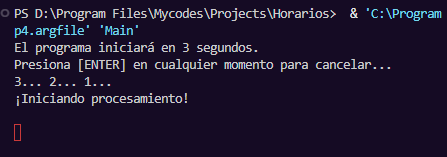
\includegraphics[width=0.8\textwidth]{img/SecuenciaArranque.png}
\end{figure}

Al final de la cuenta regresiva, el programa pide al usuario seleccionar un directorio
para guardar el archivo de salida, lo que se realiza mediante un diálogo gráfico (\texttt{JFileChooser}).

\begin{figure}[H]
    \centering
    \caption{Selección del directorio de salida mediante \texttt{JFileChooser}}
    \label{fig:file_chooser}
    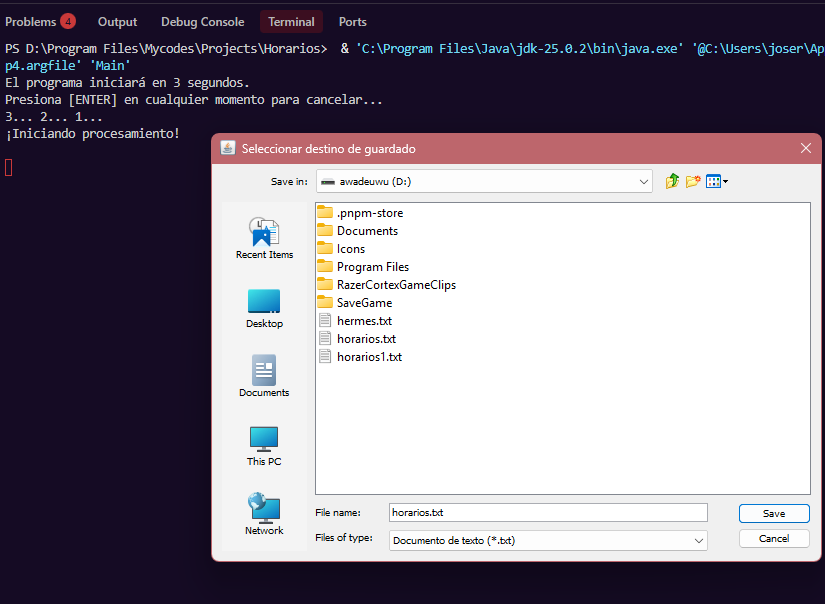
\includegraphics[width=0.8\textwidth]{img/FileChooser.png}
\end{figure}

Finalmente, el programa procede a cargar los archivos PDF desde el directorio fuente,
lo que desencadena la ejecución del programa, procesando cada documento en el orden en que son recuperados.
Tal como se muestra en la figura a continuación (figura \ref{fig:procesamiento_datos}), el programa imprime en consola el nombre de cada archivo a medida que es procesado.

\begin{figure}[H]
    \centering
    \caption{Procesamiento de datos}
    \label{fig:procesamiento_datos}
    \vspace{-0.2cm}
    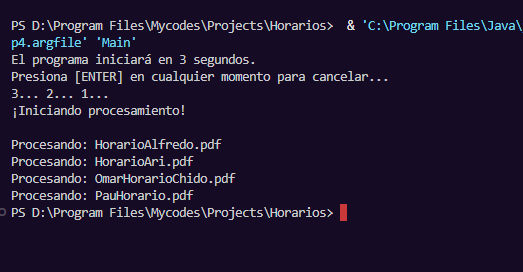
\includegraphics[width=0.8\textwidth]{img/ProcesamientoDatos.png}
\end{figure}

\subsubsection{Interrupciones}
Durante el inicio de la ejecución del programa, el hilo encargado de monitorear las entradas del teclado permanece activo,
lo que permite detectar la pulsación de la tecla \textit{Enter} en cualquier momento. Al presionar esta tecla, se genera una interrupción de software
que detiene la ejecución del programa de manera segura, asegurando que los recursos sean liberados adecuadamente y que no se produzcan estados inconsistentes.
La visualización de esta interrupción se muestra en la figura \ref{fig:interrupcion_enter}.

\begin{figure}[H]
    \centering
    \caption{Interrupción de software}
    \label{fig:interrupcion_enter}
    \vspace{-0.2cm}
    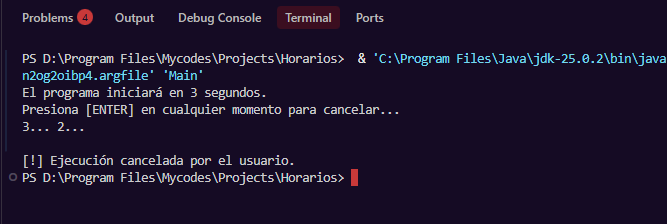
\includegraphics[width=0.8\textwidth]{img/InterrupcionEnter.png}
\end{figure}

La siguiente interrupción que se puede observar en el flujo normal es la interrupción de software generada por la cancelación
del diálogo de selección de directorio. Si el usuario decide cancelar esta acción, el programa captura esta interrupción
y detiene la ejecución de manera controlada, evitando cualquier operación posterior que dependa de la selección del directorio.
La visualización de esta interrupción se muestra en la figura \ref{fig:interrupcion_cancelar}.

\begin{figure}[H]
    \centering
    \caption{Interrupción de software por cancelación del diálogo}
    \label{fig:interrupcion_cancelar}
    \vspace{-0.2cm}
    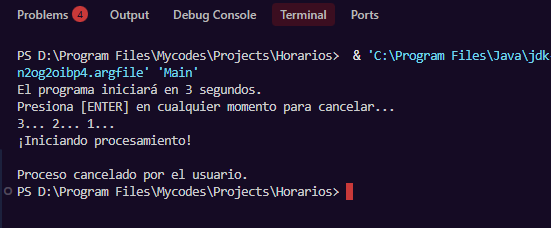
\includegraphics[width=0.8\textwidth]{img/InterrupcionFileChooser.png}
\end{figure}